% !TEX root = ../thesis.tex

\section{Results}
\label{sec:results}
This is the Results section.

\subsection{SOM Metrics}
\label{subsec:results_som_metrics}

\subsubsection{SOM-Induced Quantization}
\label{subsubsec:results_som_quantization}

heat map showing distance?

\subsubsection{Vector-Node Count}
\label{subsubsec:results_vector_node_count}

\subsubsection{Map Emptiness}
\label{subsubsec:results_map_emptiness}

\begin{figure}[!htb]
  \centering
\begin{subfigure}{0.45\textwidth}
  \centering
  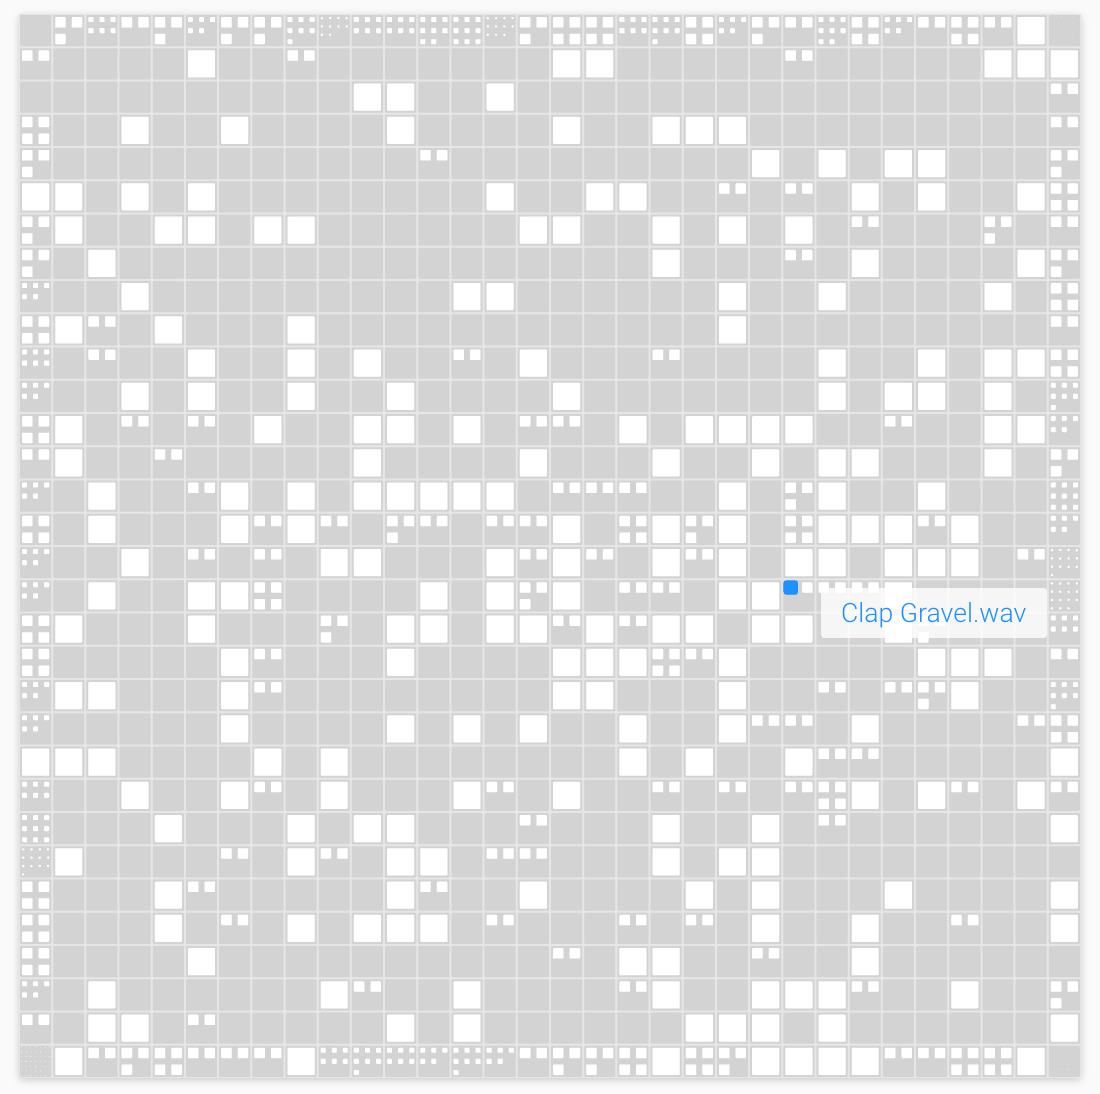
\includegraphics[width=\textwidth]{SOM-Browser_no-FNP}
  \caption{\textit{SOM Browser} without \gls{fnp}}
  \label{fig:results_no_fnp}
\end{subfigure}
~
\begin{subfigure}{0.45\textwidth}
  \centering
  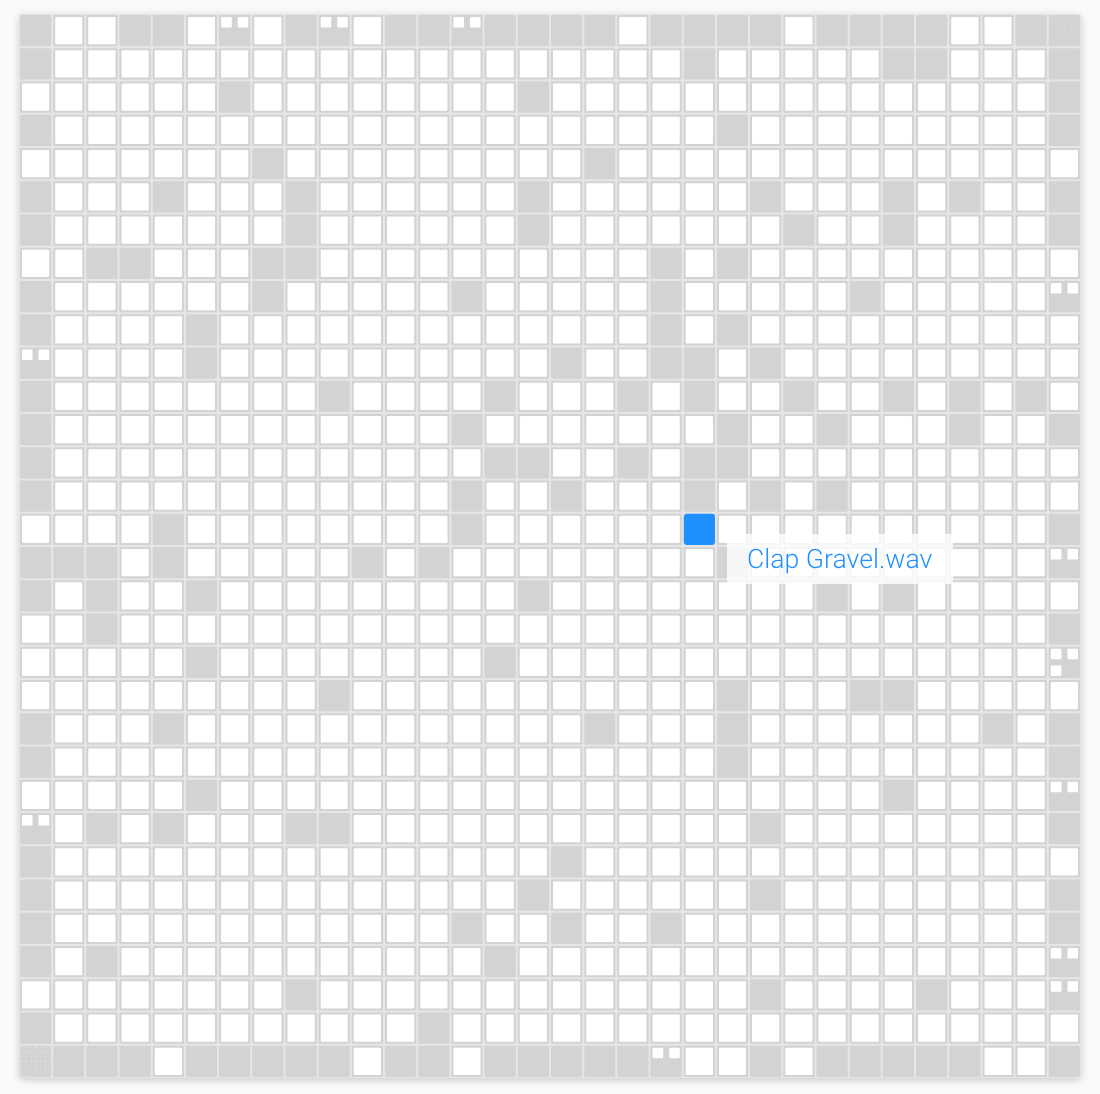
\includegraphics[width=\textwidth]{SOM-Browser_FNP}
  \caption{\textit{SOM Browser} with \gls{fnp}}
  \label{fig:results_fnp}
\end{subfigure}
\caption[\textit{SOM Browser}: Influence of FNP on Map Emptiness]
{\textit{SOM Browser}: Influence of FNP on Map Emptiness for the
\textit{Drum Essentials} sample library}
\label{fig:results_fnp_comparison}
\end{figure}


\subsection{Interview Results}
\label{subsec:results_interview}

Reference grounded theory?

code categories: cognitive, physical, perceptual, strategies, interaction style

phys: arrow keys

perceptual: colors, font size, map order

cognitive: map order, no labelled axes, overwhelming / clear interface

emergent coding vs a priori

Overview Code Tree?

% \begin{figure}[!htb]
%   \centering
% \Tree[.IP [.NP [.Det \textit{the} ]
%                [.N\1 [.N \textit{package} ]]]
%           [.I\1 [.I \textsc{3sg.Pres} ]
%                 [.VP [.V\1 [.V \textit{is} ]
%                            [.AP [.Deg \textit{really} ]
%                                 [.A\1 [.A \textit{simple} ]
%                                       \qroof{\textit{to use}}.CP ]]]]]]
% \caption{A tree caption}
% \label{table:tree_test}
% \end{figure}
%
% \forestset{
%       mathsf content/.style={content
%       format={\noexpand\ensuremath{\noexpand\mathsf{\forestoption{content}}}}},
%       }
%
% \begin{figure}[!htb]
%   \centering
%   \textbf{Established Sample Library Workflow}\par
%   \vspace{0.5cm}
%   \begin{prooftree}
%     {for tree={mathsf content}}
%     {
%       single branches
%     }
%     [, just=explan 1
%       [NP, just=explan 2
%         [Det [the]]
%         [N [cat]]
%       ]
%       [VP
%         [V [sat]]
%         [PP, just=explan 3
%           [P [on]]
%           [NP, just=explan 4
%             [Det, just=explan 5 [the, just=explan 6]]
%             [N [mat]]
%           ]
%         ]
%       ]
%     ]
%   \end{prooftree}
% \caption{A tree caption}
% \label{table:results_current_workflow}
% \end{figure}

Based on questions 1 - 2:

cite \citet{saldana2015}

\begin{figure}[!htb]
  \centering
  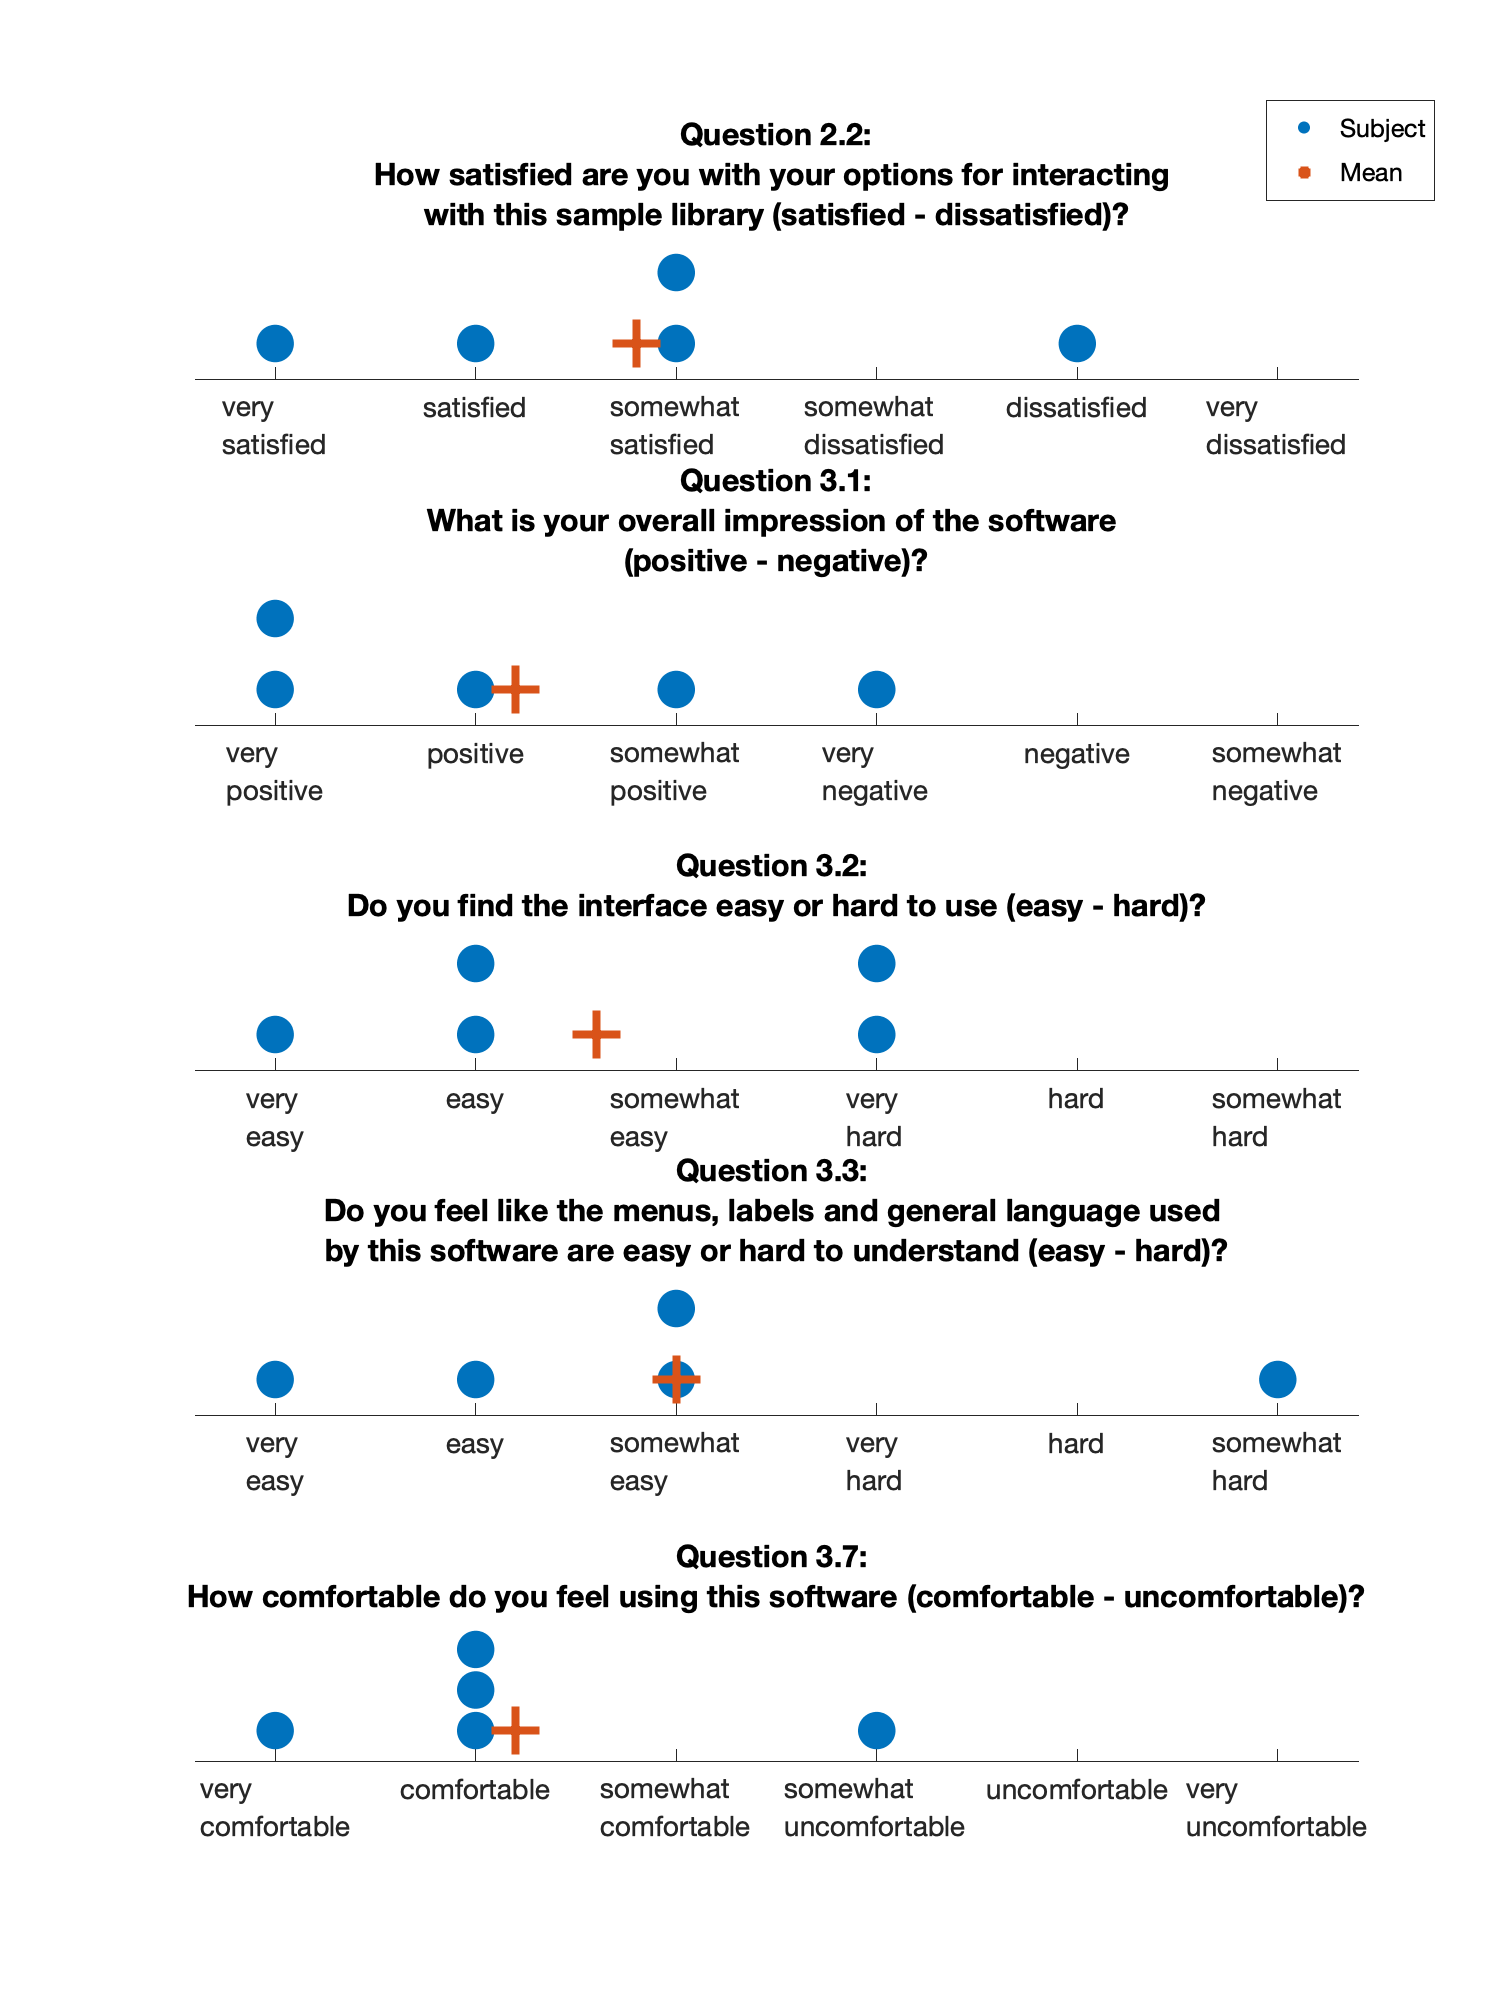
\includegraphics[width=\linewidth, trim = 25mm 10mm 10mm 10mm, clip]
  {eval_ratings}
  \caption[Interview Ratings]{Likert scale ratings by interview subjects for
  questions concerning satisfaction with their current sample library workflow
  and first \textit{SOM Browser} impressions}
  \label{fig:results_ratings}
\end{figure}

\clearpage

\begin{table}[!htb]
  \textbf{Description of Established Sample Library Workflow}
  \renewcommand{\arraystretch}{1.2}
  \centering
  \footnotesize
  % \rowcolors{2}{table-bg-one}{table-bg-two}
  \begin{tabular}{ p{4.0cm} p{4.75cm} p{4.75cm} }
  % \multicolumn{3}{ l }{\textbf{Question 2.1:}} \\
  % \multicolumn{3}{ p{14.5cm} }{\textbf{Imagine you were asked to familiarize
  % yourself with the presented sample library in order to use it in some of your
  % work. Can you describe how you would approach this task?}} \\
  % \multicolumn{3}{ p{14.5cm} }{\normalsize{\textbf{Description of Established
  % Sample Library Workflow}}} \\
  \hline
    \textbf{Code} & \textbf{Example} & \textbf{Summary} \\
    \hline
    \textbf{Mental Representation}
    &
    "I know exactly what I'm looking for"
    &
    Subjects often have a clear \textbf{mental representation} of the sound they
    are searching.
    \\
    \textbf{Goal Pursuit}
    &
    [I listen to sounds] "[u]ntil I find the one that I want"
    &
    Subjects will only look for sounds until they find something that satisfies
    their immediate needs.
    \\
    \textbf{Search Algorithm}
    &
    "I would just go through every folder [...] and listen carefully to every
    sound"
    &
    Subjects describe three \textbf{search "algorithms"}: sequential
    (listening in alphabetical order), name-based (looking at file or subfolder
    names) and random search (arbitrarily selecting samples).
    \\
    \textbf{Contextual Evaluation}
    &
    "quickly go through the sounds while the track is playing and then find
    one that kind of fits"
    &
    The ability to audition sounds in the \textbf{context} of the relevant
    project is important.
    \\
    \textbf{Iteration}
    &
    "I will have like eight different kick drums [...] and then I go through
    them again as another iteration of choice."
    &
    Subjects will select a variety of samples as potential candidates and then
    perform another search among the selected subset.
    \\
    \textbf{Frustration}
    &
    "it takes a lot of time actually and it's not the most fun part"
    &
    Looking through lists of samples sequentially is perceived to cause
    \textbf{frustration}.
    \\
  \end{tabular}
  \caption[Established Sample Library Workflow Description: Response Codes]
  {Established sample library workflow as described by subjects. Shown are
  response codes along with example data and interpretive summary.}
  \label{table:current_workflow_description}
\end{table}

Flowchart of workflow based on Table \ref{table:current_workflow_description}:

\begin{figure}[!htb]
  \centering
  \begin{tikzpicture}[node distance=3mm,
    box/.style={
      rectangle, text centered, rounded corners,
      minimum width = 5cm, minimum height = 2cm,
      fill=table-bg-two, text width=5cm
    },
    item/.style={
      rectangle, text centered, rounded corners, font=\footnotesize,
      minimum width = 3cm, minimum height = 1cm,
      fill=table-bg-two, text width=3cm
    },
    arrow/.style={
      thick,->,>=stealth
    }
  ]
  % \tikzstyle{every node}=[font=\footnotesize]

  \node (well_defined) [item] {Well-Defined};
  \node (ambiguous) [item, below = of well_defined] {Ambiguous};
  \node (os) [item, below = 6mm of ambiguous] {\gls{os} File Browser};
  \node (daw) [item, below = of os] {\gls{daw} Browser};
  \node (sequential) [item, below = 6mm of daw] {Sequential};
  \node (name_based) [item, below = of sequential] {Name-Based};
  \node (random) [item, below = of name_based] {Random};
  \node (match) [item, below = 6mm of random] {Match};
  \node (iteration) [item, below = of match] {Iteration};

  \path (well_defined.west)-- coordinate (aux1) (ambiguous.west);
  \node (mental_representation) [box, left = 6mm of aux1]
  {Mental Representation \\of Sound};

  \path (os.west)-- coordinate (aux2) (daw.west);
  \node (tool) [box, left = 6mm of aux2] {Search Tool};

  \node(algorithm) [box, left = 6mm of name_based] {Search Algorithm};

  \path (match.west)-- coordinate (aux3) (iteration.west);
  \node (evaluation) [box, left = 6mm of aux3] {Contextual Evaluation};

  \draw [arrow] (mental_representation) -- (tool);
  \draw [arrow] (tool) -- (algorithm);
  \draw [arrow] (algorithm) -- (evaluation);

  \draw [arrow] (mental_representation) -- (well_defined);
  \draw [arrow] (mental_representation) -- (ambiguous);

  \draw [arrow] (tool) -- (os);
  \draw [arrow] (tool) -- (daw);

  \draw [arrow] (algorithm) -- (evaluation);
  \draw [arrow] (algorithm) -- (sequential);
  \draw [arrow] (algorithm) -- (name_based);
  \draw [arrow] (algorithm) -- (random);

  \draw [arrow] (evaluation) -- (match);
  \draw [arrow] (evaluation) -- (iteration);

  \node (ctrl1) [below = 1cm of iteration, anchor = south] {};
  \node (ctrl2) [below left = 1cm of evaluation, anchor = north] {};
  \node (ctrl3) [left = 9mm of algorithm, anchor = west] {};
  % HOLY $#&* THIS ARROW WAS A STRUGGLE TO GET STRAIGHT
  \draw [dashed, arrow] (iteration.south) -- (ctrl1.north) -- (ctrl2.east) --
  (ctrl3.east) -- (algorithm);
\end{tikzpicture}
\caption[Established sample library workflow]{Flowchart of established sample
library workflow as described by interview subjects}
\label{table:results_current_workflow}
\end{figure}

\begin{table}[!ht]
  \textbf{Assessment of Established Sample Library Workflow}
  \renewcommand{\arraystretch}{1.2}
  \centering
  \footnotesize
  % \rowcolors{2}{table-bg-one}{table-bg-two}
  \begin{tabular}{ p{4.0cm} p{4.75cm} p{4.75cm} }
  % \multicolumn{3}{ l }{\textbf{Question 2.2:}} \\
  % \multicolumn{3}{ p{14.5cm} }{\textbf{Subject Assessment of Established Sample
  % Library Workflow}} \\
  \hline
    \textbf{Code} & \textbf{Example} & \textbf{Summary} \\
    \hline
    \textbf{Requires Organization}
    &
    "if I was organized and I had my 5000 sounds from the past five years it
    [would] be really nice"
    &
    Subjects note that their current workflow relies on sample libraries that
    are organized in some way and note sources of \textbf{frustration} such as
    lost or duplicate files.
    \\
    \textbf{Requires Experience}
    &
    "experience [...] is probably the key"
    &
    \textbf{Experience} (both in a general professional sense and specific to
    the sample libraries at hand) is mentioned as a factor for an efficient,
    successful workflow.
    \\
    \textbf{Good Enough}
    &
    "It could be better but it's okay. Like, it works in most of cases."
    &
    Current workflow practices are deemed \textbf{"good enough"}, but subjects
    are interested in alternative approaches.
    \\
    \textbf{Time-Consuming}
    &
    "[H]ow to listen to all this?"
    &
    Subjects remark upon the amount of time and effort that go into searching
    through sample libraries.
    \\
    \textbf{Overwhelming}
    &
    "it was overwhelming [...] to look through all this"
    &
    Finding relevant samples in a library is described as \textbf{overwhelming}.
    \\
    \textbf{Alphabetic Bias}
    &
    "I think it makes no sense that I'm mainly choosing from the first half of
    the alphabet"
    &
    Sample selection is influenced by alphabetical name ordering. Typically,
    samples positioned towards the beginning of an alphabetical list are more
    likely to be chosen.
    \\
  \end{tabular}
  \caption[Established Sample Library Workflow Assessment: Response Codes]
  {Subjects' assessment of established sample library workflow. Shown are
  response codes along with example data and interpretive summary.}
  \label{table:current_workflow_assessment}
\end{table}

Based on questions 3.X:

if responses were mixed, they are noted in both positive and negative table

Positive + Negative Impressions

Workflow Comparison

Feature Requests

\begin{table}[!ht]
  \textbf{SOM Browser: Positive Responses}
  \renewcommand{\arraystretch}{1.2}
  \centering
  \footnotesize
  \begin{tabular}{ p{4.0cm} p{4.75cm} p{4.75cm} }
  \hline
    \textbf{Code} & \textbf{Example} & \textbf{Summary} \\
    \hline
    \textbf{Visual Design}
    &
    "Visually, it makes sense."
    &
    Subjects characterize the \textbf{visual design} of the software as
    appealing.
    \\
    \textbf{Gestural Interaction}
    &
    "for expressive gestures as a performance tool, it’s fantastic as a
    continuous thing"
    &
    Continuous playback with trackpad/mouse gestures (while holding down Shift)
    is seen positively when using \textit{SOM Browser} more like an instrument.
    \\
    \textbf{App as Instrument}
    &
    "this is an instrument"
    &
    Subjects remark upon potential creative use of the software by not just
    using it to select samples, but also treating it as an \textbf{instrument}
    by itself.
    \\
    \textbf{User-Friendly}
    &
    "Even if I would be starting, like, it's not confusing, [...] it’s clear"
    &
    Subjects describe use of the software as \textbf{user-friendly}.
    \\
    \textbf{Favorites Selection}
    &
    "I also find the favorites pretty good"
    &
    The \textit{Favorites} bar at the bottom of \textit{SOM Browser} can be seen
    as positive.
    \\
  \end{tabular}
  \caption[\textit{SOM Browser}: Positive Responses]{Positive responses given
  by subjects after using \textit{SOM Browser}. Shown are response codes along
  with example data and interpretive summary.}
  \label{table:responses_som-browser_positive}
\end{table}

\begin{table}[!ht]
  \textbf{SOM Browser: Negative Responses}
  \renewcommand{\arraystretch}{1.2}
  \centering
  \footnotesize
  \begin{tabular}{ p{4.0cm} p{4.75cm} p{4.75cm} }
  \hline
    \textbf{Code} & \textbf{Example} & \textbf{Summary} \\
    \hline
    \textbf{Incomprehensible Map Organization}
    &
    "I don't get the order, that’s frustrating."
    &
    Subjects are not able to discern any logical order within the map.
    \\
    \textbf{Usefulness}
    &
    "right now it's beautiful but it makes no sense unfortunately"
    &
    Subjects question the \textbf{usefulness} of the software in its current
    state.
    \\
    \textbf{Confused by Empty Nodes}
    &
    "Why are there a few grayed out?"
    &
    Empty nodes on the map confuse subjects.
    \\
    \textbf{Overwhelming}
    &
    "looking at these many, many tiny squares gives me anxiety"
    &
    The map interface is seen by some subjects as \textbf{overwhelming}.
    \\
    \textbf{No File Labels}
    &
    "here it’s just white bricks"
    &
    The fact that no files besides the current selection are labelled on the map
    is seen negatively by some subjects.
    \\
    \textbf{Unnecessary Interface Elements}
    &
    "Eliminate the top bar, eliminate all the bottom just keep this [points to
    map in center]"
    &
    Subjects question the need for interface elements besides the central map
    display.
    \\
  \end{tabular}
  \caption[\textit{SOM Browser}: Negative Responses]{Negative responses given
  by subjects after using \textit{SOM Browser}. Shown are response codes along
  with example data and interpretive summary.}
  \label{table:responses_som-browser_negative}
\end{table}

Special mention:

Incomprehensible Map Organization

Some recognize areas of similarity, but the overall impression is that of a
random organization.

\begin{table}[!ht]
  \textbf{Workflow Comparison: Established Workflow vs. SOM Browser}
  \renewcommand{\arraystretch}{1.2}
  \centering
  \footnotesize
  \begin{tabular}{ p{4.0cm} p{4.75cm} p{4.75cm} }
  \hline
    \textbf{Code} & \textbf{Example} & \textbf{Summary} \\
    \hline
    \textbf{Example}
    &
    "Here's an example of something someone said."
    &
    Subjects said this because they believe it to be true.
    \\
  \end{tabular}
  \caption[Workflow Comparison Established Workflow vs. \textit{SOM Browser}]
  {Subjects' responses when asked to compare their established workflows to
  \textit{SOM Browser} and state a preference. Shown are response codes along
  with example data and interpretive summary.}
  \label{table:responses_workflow_comparison}
\end{table}

\begin{table}[!ht]
  \textbf{SOM Browser: Feature Requests}
  \renewcommand{\arraystretch}{1.2}
  \centering
  \footnotesize
  \begin{tabular}{ p{4.0cm} p{4.75cm} p{4.75cm} }
  \hline
    \textbf{Code} & \textbf{Example} & \textbf{Summary} \\
    \hline
    \textbf{Example}
    &
    "Here's an example of something someone said."
    &
    Subjects said this because they believe it to be true.
    \\
  \end{tabular}
  \caption[SOM Browser: Feature Requests]{Subjects' feature requests for
  \textit{SOM Browser}. Shown are response codes along with example data and
  interpretive summary.}
  \label{table:responses_feature_requests}
\end{table}

% \begin{table}[!ht]
%   \renewcommand{\arraystretch}{1.2}
%   \centering
%   \footnotesize
%   % \rowcolors{2}{table-bg-one}{table-bg-two}
%   \begin{tabular}{ p{4.0cm} p{4.75cm} p{4.75cm} }
%   \multicolumn{3}{ l }{\textbf{Question 3.2:}} \\
%   \multicolumn{3}{ p{14.5cm} }{\textbf{Do you find the interface easy or hard to
%   use (easy - hard)? Can you elaborate on why?}} \\
%   \hline
%     \textbf{Code} & \textbf{Example} & \textbf{Summary} \\
%     \hline
%     \textbf{Example}
%     &
%     "Here's an example of something someone said."
%     &
%     Subjects said this because they believe it to be true.
%     \\
%   \end{tabular}
%   \caption[Question 3.2: Response codes]{Question 3.2: Response codes with example
%   data and interpretive summary}
%   \label{table:responses_question_3-2}
% \end{table}
%
% \begin{table}[!ht]
%   \renewcommand{\arraystretch}{1.2}
%   \centering
%   \footnotesize
%   % \rowcolors{2}{table-bg-one}{table-bg-two}
%   \begin{tabular}{ p{4.0cm} p{4.75cm} p{4.75cm} }
%   \multicolumn{3}{ l }{\textbf{Question 3.3:}} \\
%   \multicolumn{3}{ p{14.5cm} }{\textbf{Do you feel like the menus, labels and
%   general language used by this software are easy or hard to understand
%   (easy - hard)?}} \\
%   \hline
%     \textbf{Code} & \textbf{Example} & \textbf{Summary} \\
%     \hline
%     \textbf{Example}
%     &
%     "Here's an example of something someone said."
%     &
%     Subjects said this because they believe it to be true.
%     \\
%   \end{tabular}
%   \caption[Question 3.3: Response codes]{Question 3.3: Response codes with
%   example data and interpretive summary}
%   \label{table:responses_question_3-3}
% \end{table}
%
% \begin{table}[!ht]
%   \renewcommand{\arraystretch}{1.2}
%   \centering
%   \footnotesize
%   % \rowcolors{2}{table-bg-one}{table-bg-two}
%   \begin{tabular}{ p{4.0cm} p{4.75cm} p{4.75cm} }
%   \multicolumn{3}{ l }{\textbf{Question 3.4:}} \\
%   \multicolumn{3}{ p{14.5cm} }{\textbf{What do you think about the organization
%   of sounds in this interface?}} \\
%   \hline
%     \textbf{Code} & \textbf{Example} & \textbf{Summary} \\
%     \hline
%     \textbf{Example}
%     &
%     "Here's an example of something someone said."
%     &
%     Subjects said this because they believe it to be true.
%     \\
%   \end{tabular}
%   \caption[Question 3.4: Response codes]{Question 3.4: Response codes with
%   example
%   data and interpretive summary}
%   \label{table:responses_question_3-4}
% \end{table}
%
% \begin{table}[!ht]
%   \renewcommand{\arraystretch}{1.2}
%   \centering
%   \footnotesize
%   % \rowcolors{2}{table-bg-one}{table-bg-two}
%   \begin{tabular}{ p{4.0cm} p{4.75cm} p{4.75cm} }
%   \multicolumn{3}{ l }{\textbf{Question 3.5:}} \\
%   \multicolumn{3}{ p{14.5cm} }{\textbf{What do you think the axes represent?}} \\
%   \hline
%     \textbf{Code} & \textbf{Example} & \textbf{Summary} \\
%     \hline
%     \textbf{Example}
%     &
%     "Here's an example of something someone said."
%     &
%     Subjects said this because they believe it to be true.
%     \\
%   \end{tabular}
%   \caption[Question 3.5: Response codes]{Question 3.2: Response codes with
%   example data and interpretive summary}
%   \label{table:responses_question_3-5}
% \end{table}
%
% \begin{table}[!ht]
%   \renewcommand{\arraystretch}{1.2}
%   \centering
%   \footnotesize
%   % \rowcolors{2}{table-bg-one}{table-bg-two}
%   \begin{tabular}{ p{4.0cm} p{4.75cm} p{4.75cm} }
%   \multicolumn{3}{ l }{\textbf{Question 3.6:}} \\
%   \multicolumn{3}{ p{14.5cm} }{\textbf{Which do you prefer: the map layout or a
%   traditional file manager interface and folder structure (or a combination of
%   both)?}} \\
%   \hline
%     \textbf{Code} & \textbf{Example} & \textbf{Summary} \\
%     \hline
%     \textbf{Example}
%     &
%     "Here's an example of something someone said."
%     &
%     Subjects said this because they believe it to be true.
%     \\
%   \end{tabular}
%   \caption[Question 3.6: Response codes]{Question 3.6: Response codes with
%   example data and interpretive summary}
%   \label{table:responses_question_3-6}
% \end{table}
%
% \begin{table}[!ht]
%   \renewcommand{\arraystretch}{1.2}
%   \centering
%   \footnotesize
%   % \rowcolors{2}{table-bg-one}{table-bg-two}
%   \begin{tabular}{ p{4.0cm} p{4.75cm} p{4.75cm} }
%   \multicolumn{3}{ l }{\textbf{Question 3.7:}} \\
%   \multicolumn{3}{ p{14.5cm} }{\textbf{How comfortable do you feel using this
%   software (comfortable - uncomfortable)?}} \\
%   \hline
%     \textbf{Code} & \textbf{Example} & \textbf{Summary} \\
%     \hline
%     \textbf{Example}
%     &
%     "Here's an example of something someone said."
%     &
%     Subjects said this because they believe it to be true.
%     \\
%   \end{tabular}
%   \caption[Question 3.7: Response codes]{Question 3.7: Response codes with
%   example data and interpretive summary}
%   \label{table:responses_question_3-7}
% \end{table}
%
% \begin{table}[!ht]
%   \renewcommand{\arraystretch}{1.2}
%   \centering
%   \footnotesize
%   % \rowcolors{2}{table-bg-one}{table-bg-two}
%   \begin{tabular}{ p{4.0cm} p{4.75cm} p{4.75cm} }
%   \multicolumn{3}{ l }{\textbf{Question 3.8:}} \\
%   \multicolumn{3}{ p{14.5cm} }{\textbf{Would you consider using this tool in the
%   future or not? If not, what changes would you like to see?}} \\
%   \hline
%     \textbf{Code} & \textbf{Example} & \textbf{Summary} \\
%     \hline
%     \textbf{Example}
%     &
%     "Here's an example of something someone said."
%     &
%     Subjects said this because they believe it to be true.
%     \\
%   \end{tabular}
%   \caption[Question 3.8: Response codes]{Question 3.8: Response codes with
%   example data and interpretive summary}
%   \label{table:responses_question_3-8}
% \end{table}
